\documentclass[tikz,border=10pt]{standalone}
\usepackage{tikz}
\usepackage{amssymb}
\usepackage{amsmath}
\usetikzlibrary{positioning, arrows.meta, shapes.geometric, shapes.misc,
                shapes.multipart, backgrounds, fit, calc}

\begin{document}
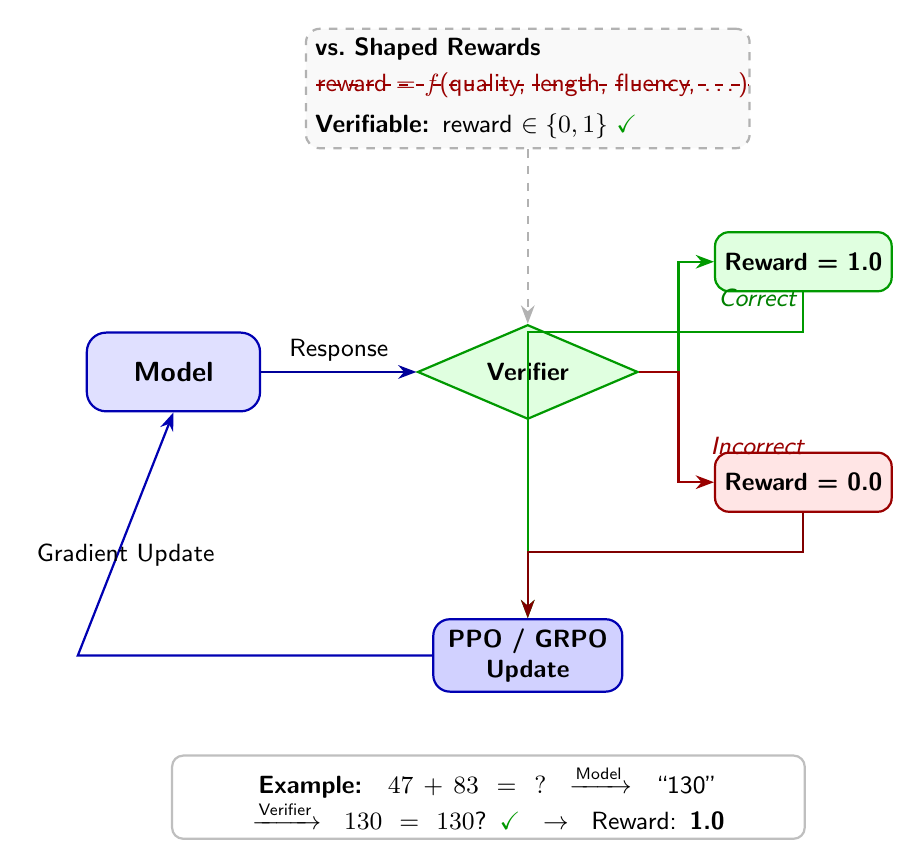
\begin{tikzpicture}[
  font=\sffamily,
  >=Stealth,
  thick,
  %% Main node styles
  model/.style={
    draw=blue!70!black, fill=blue!12, rounded corners=7pt, thick,
    minimum width=2.2cm, minimum height=1.0cm, align=center,
    font=\sffamily\bfseries
  },
  verifier/.style={
    draw=green!60!black, fill=green!12, thick,
    shape=diamond, aspect=1.8,
    minimum width=2.8cm, minimum height=1.2cm, align=center,
    font=\sffamily\bfseries\small
  },
  reward-good/.style={
    draw=green!60!black, fill=green!12, rounded corners=5pt, thick,
    minimum width=2.2cm, minimum height=0.75cm, align=center,
    font=\sffamily\bfseries\small
  },
  reward-bad/.style={
    draw=red!60!black, fill=red!10, rounded corners=5pt, thick,
    minimum width=2.2cm, minimum height=0.75cm, align=center,
    font=\sffamily\bfseries\small
  },
  update/.style={
    draw=blue!70!black, fill=blue!18, rounded corners=6pt, thick,
    minimum width=2.4cm, minimum height=0.85cm, align=center,
    font=\sffamily\bfseries\small
  },
  %% Annotation / example box styles
  annotation/.style={
    draw=gray!60, fill=gray!5, rounded corners=5pt, dashed, thick,
    align=left, font=\sffamily\small
  },
  example/.style={
    draw=gray!50, fill=white, rounded corners=4pt, thick,
    align=center, font=\sffamily\small
  },
]

%% ── MAIN NODES ────────────────────────────────────────────────────────────
\node[model]    (model)    at (0, 0)      {Model};
\node[verifier] (verifier) at (4.5, 0)    {Verifier};
\node[reward-good] (r1)    at (8.0,  1.4) {Reward = 1.0};
\node[reward-bad]  (r0)    at (8.0, -1.4) {Reward = 0.0};
\node[update]   (update)   at (4.5, -3.6) {PPO / GRPO\\Update};

%% ── MAIN ARROWS ───────────────────────────────────────────────────────────
%% Model → Verifier
\draw[->, thick, blue!60!black]
  (model.east) -- (verifier.west)
  node[midway, above, font=\sffamily\small, black] {Response};

%% Verifier → Reward=1.0 (correct path)
\draw[->, thick, green!60!black]
  (verifier.east) -- ++(0.5,0) |- (r1.west)
  node[near start, above, font=\sffamily\small\itshape, xshift=1.0cm, green!50!black] {Correct};

%% Verifier → Reward=0.0 (incorrect path)
\draw[->, thick, red!60!black]
  (verifier.east) -- ++(0.5,0) |- (r0.west)
  node[near start, below, font=\sffamily\small\itshape, xshift=1.0cm, red!60!black] {Incorrect};

%% Reward=1.0 → Update
\draw[->, thick, green!60!black]
  (r1.south) -- ++(0,-0.5cm) -| (update.north);

%% Reward=0.0 → Update
\draw[->, thick, red!50!black]
  (r0.south) -- ++(0,-0.5cm) -| (update.north);

%% Update → Model (feedback loop, below)
\draw[->, thick, blue!70!black]
  (update.west) -- ++(-4.5, 0) -- (model.south)
  node[midway, below, font=\sffamily\small, black] {Gradient Update};

%% ── COMPARISON ANNOTATION ─────────────────────────────────────────────────
\node[annotation, text width=5.4cm] (annot) at (4.5, 3.6) {
  \textbf{vs.\ Shaped Rewards}\\[2pt]
  \textcolor{red!60!black}{%
    \tikz[baseline=(t.base)]{%
      \node[inner sep=0pt] (t) {reward = $f$(quality, length, fluency, \ldots)};%
      \draw[red!60!black, thick] (t.west) -- (t.east);%
    }%
  }\\[4pt]
  \textbf{Verifiable:} reward $\in \{0, 1\}$ \textcolor{green!60!black}{$\checkmark$}
};

%% Arrow from annotation to verifier
\draw[->, dashed, gray!60] (annot.south) -- (verifier.north);

%% ── EXAMPLE BOX ───────────────────────────────────────────────────────────
\node[example, text width=7.8cm] (example) at (4.0, -5.4) {
  \textbf{Example:}\quad
  $47 + 83 = \;?$
  \;\;$\xrightarrow{\text{Model}}$\;\;
  ``130''
  \;\;$\xrightarrow{\text{Verifier}}$\;\;
  $130 = 130$? \textcolor{green!60!black}{$\checkmark$}
  \;\;$\to$\;\;
  Reward: \textbf{1.0}
};

\end{tikzpicture}
\end{document}
